\documentclass{article}
\usepackage[utf8]{inputenc}
\usepackage[spanish]{babel} 
\renewcommand{\spanishtablename}{Tabla} 
\spanishdecimal{.}
\usepackage{verbatim}
\usepackage{amssymb}
\usepackage{wrapfig}
\usepackage{graphicx}
\usepackage{mathtools}
\usepackage{subfig}
\usepackage{float}
\usepackage{siunitx}
\renewcommand{\thefootnote}{\arabic{fotnote}}
\setlength{\parskip}{\baselineskip} 
\usepackage{pdfpages}

\begin{document}

\begin{titlepage}

\begin{center}
\vspace*{0.10in}
\begin{figure}
\raggedleft

\includegraphics[scale=0.12]{unam.png}
\hspace{7.2cm}
\raggedright

\includegraphics[scale=0.15]{fac.png}    
\end{figure}
\vspace*{0.5in}
UNIVERSIDAD NACIONAL AUTÓNOMA DE MÉXICO\\
\vspace*{0.2in}
FACULTAD DE CIENCIAS \\
\vspace*{0.5in}
\begin{large}
Laboratorio de Calor, Ondas y Fluidos\\
\end{large}
\vspace*{0.2in}
\begin{Large}
\textbf{Práctica 1} \\
\textbf{Calibración de un Termómetro.} \\
\end{Large}
\vspace*{0.3in}
\vspace*{0.3in}
\rule{80mm}{0.1mm}\\
\vspace*{0.1in}
\begin{large}
Profesor:  Quintanar Robles, Luis  \\
Ayudante: Quintanar Cortés, Luis Enrique \\
Mesa 1\\
Alumnos: León Arenal Sebastian.\\
Robledo Ibarra Emiliano. \\
Toledo Castañeda, Akim Tarik.\\


\end{large}
\end{center}
\end{titlepage}
\section*{Resumen.}
Se construyeron dos termómetros utilizando un matraz, un capilar y agua; mediante el mismo se buscó una relación lineal entre el cambio de la temperatura y la longitud de la columna de agua dentro del capilar y así poder medir la temperatura aprovechando el equilibrio térmico y transferencia de calor. En lo referente a la escala termométrica se encontraron rectas paralelas pero con ordenadas al origen distintas para cada termómetro.

\section*{Introducción.} 
Saber la temperatura a la que se encuentra algún cuerpo es fundamental en el estudio de la termodinámica. Para determinar temperaturas generalmente se ocupa un termómetro; este instrumento de medición relaciona cambios entre propiedades físicas de una sustancia termométrica, donde una de estas propiedades cambia con la temperatura. Por ejemplo, el termómetro de mercurio relaciona el cambio en la temperatura con la expansión volumétrica de este metal. Cuando el mercurio se calienta y se expande, este asciende por su contenedor. Se escala el termómetro en base a un cambio en la longitud de la columna de mercurio respecto al cambio de la temperatura. Sin embargo, en este tipo de termómetros, la escala de temperatura dependerá de la sustancia termométrica y de un punto de partida arbitrario; por ejemplo, la escala Celsius tiene su cero en la temperatura asociada al punto de fusión del agua y su 100 en el punto de ebullición de la misma. En este experimento se construyó un termómetro cuya sustancia termométrica era agua. Se relacionaron, linealmente, el cambió en la temperatura y el cambio en las alturas asociadas a ellas.\\ 
 El objetivo del experimento es construir un termómetro que relacione, linealmente, la temperatura del agua dentro de un matraz y la longitud de la columna de agua que sube por un capilar unido al matraz. La práctica consistió en medir qué tanto subió el agua dentro del capilar al incrementar la temperatura exterior del matraz con el fin de obtener una relación entre el cambio de temperatura y la altura del agua dentro del capilar.
 Se formuló la siguiente hipótesis: conforme suba la temperatura, la columna de agua que sube por el capilar será mas grande. La relación entre los cambios de temperatura y altura es lineal. Algunas hipótesis extras como la dilatación de la sustancia termométrica es lineal y además el agua dentro del termómetro adopta una temperatura igual después de cinco minutos de reposo.

\section*{Procedimiento.}
En la práctica se imitó el funcionamiento de un termómetro: lo primero que se buscó fue una sustancia termométrica y posteriormente un sistema con esta dentro. Se llenó con agua un matraz de 25 mL a máxima capacidad y se selló con un tapón de hule con un capilar largo de vidrio atravesándolo para que con este capilar se establecieran las marcas que funcionarían de escala posteriormente; establecido el sistema a usar, se resalta que este mismo se encuentra eliminando toda consideración de las diferentes expansiones del agua y que estas son lineales puesto que el termómetro también lo es.  A continuación, se llamará  a este sistema como: "termómetro experimental". El termómetro experimental se consideró con un límite debido a la sustancia termométrica, este fue limitar la temperatura mínima del agua a la cual se mediría un cambio.

\begin{figure}[H]
    \centering
    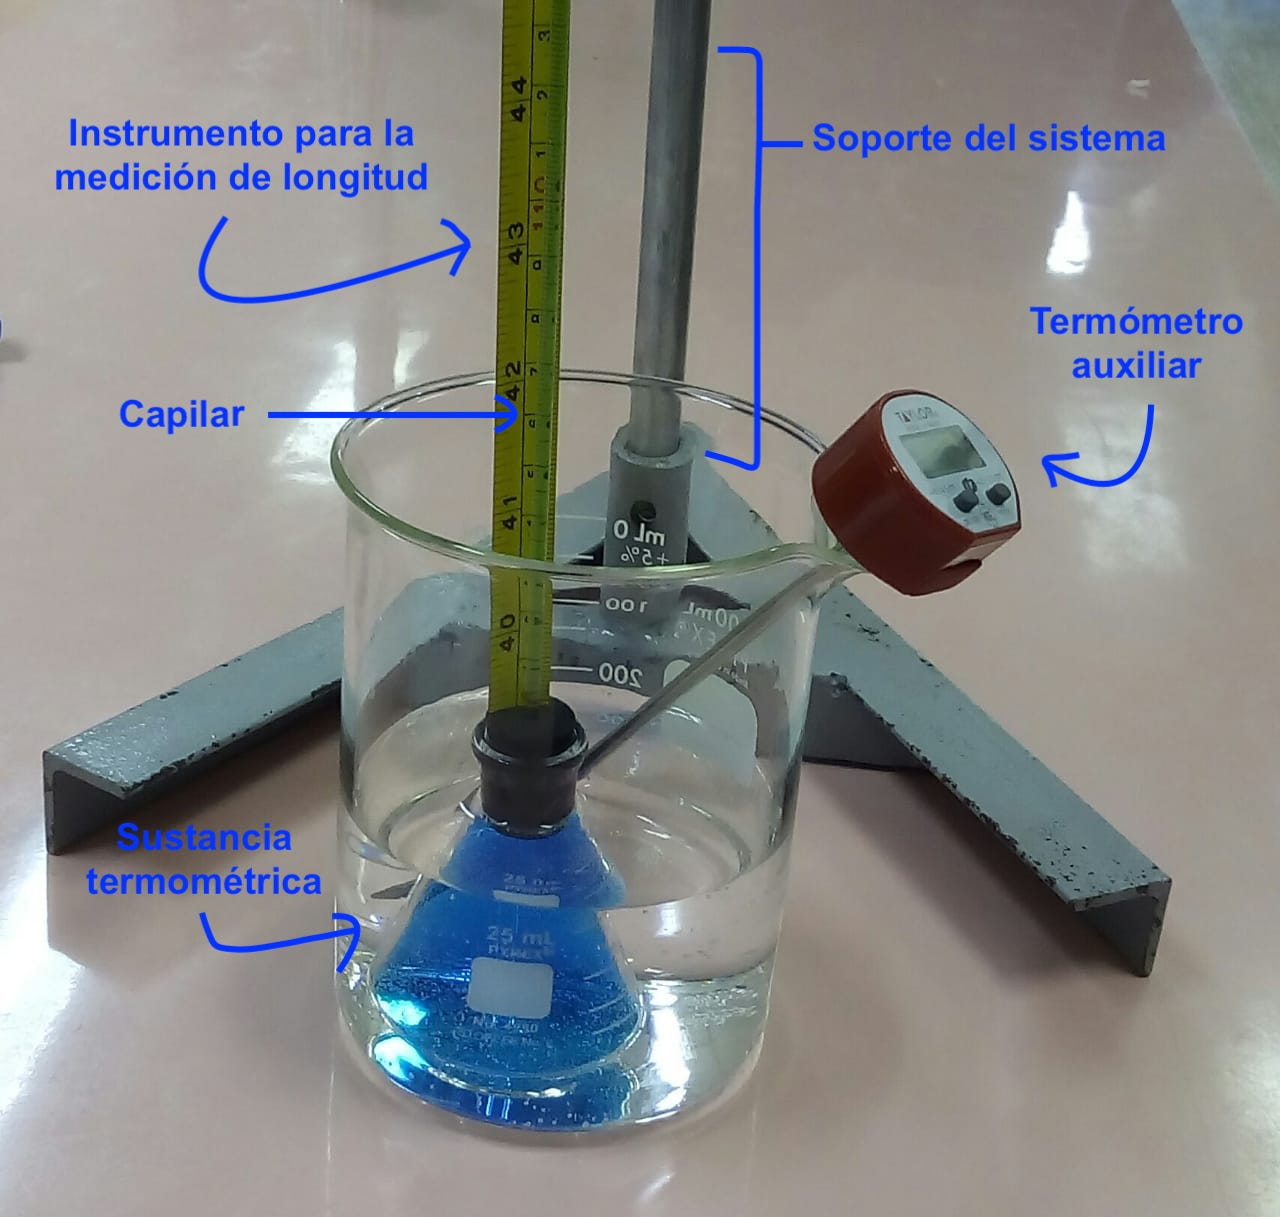
\includegraphics[width=9cm]{Sistema.jpeg}%
    \caption{Diagrama del sistema empleado con sus partes.}%
\end{figure}

Se vertió agua en un vaso de precipitado de 500 mL a temperatura ambiente a una altura necesaria para que todo el matraz de nuestro termómetro se viera rodeado de agua y una vez cumplido dicho requerimiento se colocó el termómetro experimental dentro; una vez hecho esto, se optó por esperar 5 minutos  para que la columna de agua se estabilizara en una altura, posterior a ello se registró la temperatura del agua en el recipiente e etiquetó como temperatura inicial ($T_{i1}$) con su respectiva altura de la columna de agua que subió por el capilar. La medición se realizó tomando en cuenta la parte de arriba del tapón como el origen. A la longitud de la columna de agua se le registró como longitud inicial ($L_{i1}$) a manera de obtención de la primera pareja $(L_{i1} , T_{i1})$. Después de registrar las condiciones iniciales, que servirían de medida básica para la formulación de una escala del termómetro experimental, éste se removió del vaso de precipitado. Se calentó el agua dentro del vaso de precipitado con una parrilla eléctrica y una vez que el agua dentro del contenedor alcanzó los 55$^{\circ}$C  se repitió el proceso de medición, esto es, se colocó el termómetro experimental en contacto con el líquido al cual se le elevó la temperatura y una vez esperados cinco minutos se tomo la dupla de temperatura del agua y matraz con la altura a la cual el capilar permaneció estable. Al haber esperado el tiempo de estabilización, se usó un termómetro digital como referencia para así poder establecer la segunda dupla con temperatura de 51.8$^{\circ}$C, de manera que de esta segunda medición se obtuvo:  ($L_{f1}$ , $T_{f1}$).

Para comprobar la reproducibilidad del termómetro experimental se diseño uno con las mismas características junto con las mismas técnicas de medición y a partir de dicho procedimiento se obtuvieron valores $L_{i2}$ y $L_{f2}$ para la longitud de la columna de agua y $T_{i2}$,$T_{f2}$ para las temperaturas. Gracias a las medidas obtenidas de ambos termómetros se obtuvieron dos rectas que se esperaría que fueran iguales.

Cada termómetro fue sensible a los factores en los cuales se armó; sin embargo, se buscó que el dispositivo no se viera afectado por factores de ensamblaje. La única diferencia trascendental se llevó a cabo en la fuerza aplicada para sellar el sistema. Debido a esto, las alturas iniciales de cada termómetro variaron; sin embargo, se consideró que esto no afectaría en sobremanera a la escala termométrica posteriormente formulada obtenida como:

$$T_{x}=\frac{(L_{x}-L_{i})\Delta T}{\Delta L} + T_{i}$$

En ella se expresó la relación entre una nueva medida y las dos que sirvieron de base a una escala termométrica, para poder usarla se consideraron dos factores importantes que definieron una hipótesis:

\begin{itemize}
    \item La relación entre los datos que se obtuvieron puede ser reducida a una relación lineal.
    \item La pendiente de dicha formulación se mantiene constante, es decir, siempre es una recta para las temperaturas consideradas en el dominio de la función.
\end{itemize}

Al formular una relación lineal, se cuenta con una pendiente que muestra el núcleo de dicha función: $m = \frac{\Delta T}{\Delta L} = \frac{T_f - T_i }{L_f - L_i}$ podemos ver que al ser $\Delta T$ un número obtenido por medio de mediciones directas de temperatura su incertidumbre constó de la suma de las incertidumbres individuales esto es: $d \Delta T = 0.1^{\circ}C$. Análogamente, para las alturas obtenidas se consideró: $d \Delta L = 0.1 cm$.


\section*{Resultados.}
Se registraron los siguientes datos para el primer termómetro:

\begin{table}[H]
  \centering
    \begin{tabular}{|c|c|} \hline
    
    Temperatura inicial [$T_{i1}$] & 22.4 $^{\circ}$C \\ \hline
    Longitud inicial [$L_{i1}$]     & 27.2 cm\\ \hline
    Temperatura final [$T_{f1}$]    & 51.8 $^{\circ}$C \\ \hline
    Longitud final [$L_{f1}$]     & 41 cm \\ \hline
    
    \end{tabular}%
\caption{Datos del Termómetro 1 $d T=\pm 0.05^{\circ}C ; d L=\pm 0.05cm$}


\end{table}%


\begin{table}[H]
  \centering
    \begin{tabular}{|c|c|} \hline
    Temperatura inicial [$T_{i2}$] & 22.3  $^{\circ}$C \\ \hline
    Longitud inicial [$L_{i2}$]    & 22.7 cm\\ \hline
    Temperatura final [$T_{f2}$]    & 36.3 $^{\circ}$C \\ \hline
    Longitud final [$L_{f2}$]     & 29.1 cm \\ \hline
    
    \end{tabular}%
\caption{Datos del Termómetro 2 $d T= \pm 0.05^{\circ}C ;  dL = \pm 0.05cm$}


\end{table}%

Suponiendo una relación lineal entre el cambio en la temperatura y el cambio en la longitud de la columna de agua, se obtiene:
$$T_{x}=\frac{(L_{x}-L_{i})\Delta T}{\Delta L} + T_{i}$$
Donde $\Delta T = (T_{f}-T_{i})$ ; $\Delta L = (L_{f}-L_{i})$; $T_{x}$ es la temperatura asociada a una longitud $L_{x}$

 \begin{figure}[H]%
    \centering
    \subfloat[$f(x) = 2.1x-35.5$]{{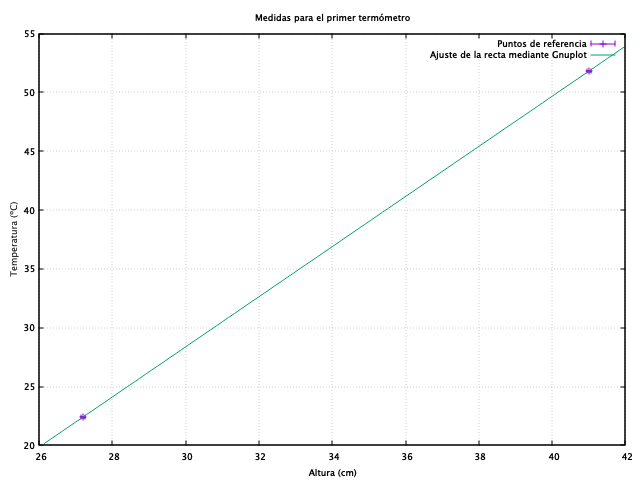
\includegraphics[width=5.5cm]{Term1.png} }}%
    \qquad
    \subfloat[$f(x) = 2.2x-27.4$]{{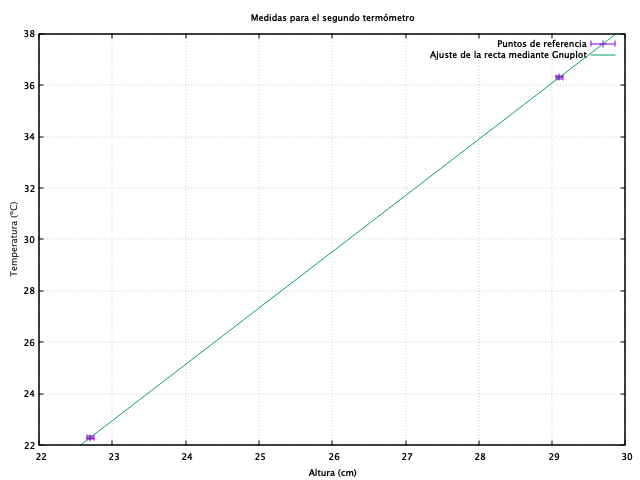
\includegraphics[width=5.5cm]{Term2Gnuplot.png} }}%
    \caption{Ajuste en gnuplot para ambos termómetros.}%
    \label{fig:example}%
\end{figure}

Y la incertidumbre asociada es: 

$$\partial T_x = \left| \frac{L_x - L_i}{\Delta L} \right| d\Delta T + \left| - \frac{(L_x - L_i) \Delta T}{\Delta L^2} \right| d\Delta L + \left| \frac{\Delta T}{\Delta L} \right| d(L_x - L_i) + dT_i $$

Se observa en el ajuste de Gnuplot que las pendientes del las rectas asociadas a cada termómetro son prácticamente iguales. Esto era de esperarse, pues la sustancia en cada termómetro era la misma. En ambos termómetros se tienen condiciones iniciales de temperatura distintas por una décima de grado, sin embargo, las longitudes iniciales sí difieren bastante. A esta diferencia se le atribuye que no sean iguales las ordenadas al origen de ambas rectas. El cociente entre el cambio de temperatura y el cambio en la longitud fue el mismo incluso con la diferencia de las longitudes iniciales. Suponiendo que la relación es lineal, sería imposible que a temperaturas diferentes por décimas de grado se atribuyan diferencias de unidades en la longitud. Esta discrepancia en las longitudes iniciales se puede deber a un mal armado de algún termómetro. Tal vez, alguno de los dos no se selló bien con el tapón o, quizás, alguno no se llenó completamente de agua. 


\section*{Conclusiones}
\begin{itemize}
    \item No es posible que aseguremos que la relación entre la realidad y  el modelo creado sea lineal, debido a que sólo dos puntos fueron tomados como referencia y de ello podría haber una relación no lineal. Para garantizar el comportamiento deseado se deben registrar múltiples puntos utilizando el mismo termómetro.
    \item Para obtener una mejor aproximación en las gráficas hacen falta más datos. Los cuales no fueron posibles de obtener debido se consumió bastante tiempo preparando otro termómetro con una sustancia termométrica distinta que, al final, no se utilizó.
    \item La sustancia termométrica utilizada tardó mucho tiempo en estar en equilibrio térmico. Las medidas consumieron mucho tiempo por este motivo. El experimento se puede agilizar utilizando una sustancia que responda más rápido a los cambios de temperatura. Por ejemplo, alcohol.
    \item Las pendientes de las rectas de cada termómetro coinciden por que se utilizó la misma sustancia termométrica. Las ordenadas al origen son diferentes por un error experimental provocado por la construcción inexacta del sistema que es de hecho la presurización del sistema y la temperatura inicial del agua dentro del matraz. La diferencia entre las temperaturas iniciales y sus longitudes se hace notar en la discrepancia de las ordenadas al origen. Se esperaban dos rectas paralelas; esto se cumplió al observar pendientes asociadas de 2.1 y 2.2. Sin embargo, no se puede afirmar que sean la misma recta pues la ordenadas al origen difieren en 8.1 unidades. Ni siquiera las incertidumbres excusan esta diferencia.
    \item El sistema del termómetro puede mejorar en cuanto a su intercambio de energía, el vidrio pyrex es hecho de manera que soporte altas temperaturas por lo cual puede representar un problema en cuanto a la estabilización de la columna de agua que funciona de guía para el termómetro. 

\end{itemize}

\begin{figure}[H]%
    \centering
    \subfloat[$f(x) = 2.1x-35.5$]{{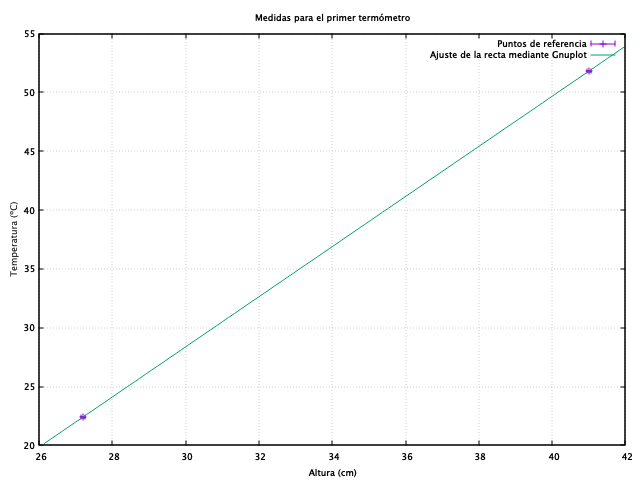
\includegraphics[width=12cm]{Term1.png} }}%
    \qquad
    \subfloat[$f(x) = 2.2x-27.4$]{{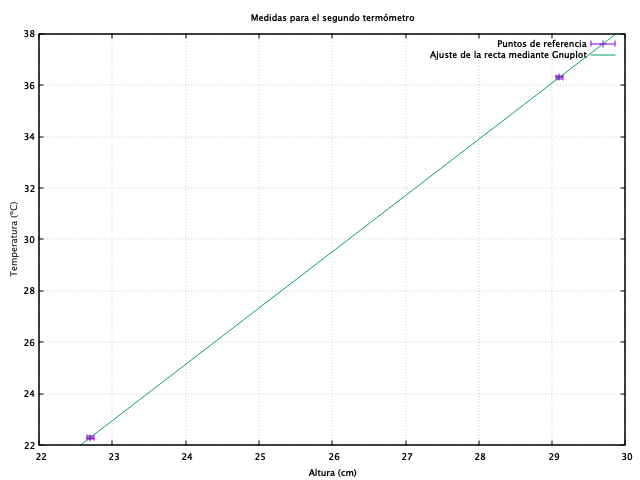
\includegraphics[width=12cm]{Term2Gnuplot.png} }}%
    \caption{Ajuste en gnuplot para ambos termómetros.}%
    \label{fig:example}%
\end{figure}



\end{document}
